\documentclass{article}[12pt]

\usepackage{amsthm}
\usepackage{amssymb}
\usepackage{amsmath}
\usepackage{mathtools}

%\usepackage{fontspec}
\usepackage[margin=1in]{geometry}
\setlength{\parindent}{0pt}

\usepackage{indentfirst}
\usepackage{setspace}
\usepackage{graphicx}
\usepackage{wrapfig}
\usepackage{caption}
\usepackage{subcaption}
\usepackage{siunitx}

%\setmainfont{Helvetica}

\theoremstyle{definition}
\newtheorem{theorem}{Theorem}
\newtheorem{definition}[theorem]{Definition}
\newtheorem*{theorem*}{Theorem}

\newcommand{\myabs}[1]{\vert#1\vert}
\newcommand{\pder}[2]{\frac{\partial#1}{\partial#2}}
\newcommand{\pdder}[2]{\frac{\partial^2#1}{\partial#2^2}}
\newcommand{\dder}[2]{\frac{d^2#1}{d^2#2}}
\newcommand{\orb}{\mathcal{O}}

\DeclareMathOperator{\iso}{Iso}
\DeclareMathOperator{\fix}{Fix}
\DeclareMathOperator{\tr}{Tr}
\DeclareMathOperator{\vol}{vol}

\begin{document}
\singlespacing
\title{Hearing the Local Orientability of Orbifolds}
\author{Sean Richardson}
\date{\today}
\maketitle

\begin{abstract}
    Given a drum, a skilled mathematician can deduce what sound the drum
    will make when hit. But consider the reverse: if a mathematician heard
    the drum in a neighboring room, could they reverse engineer the shape
    of the drum.  Mark Kac elegantly framed this question as: ``can you
    hear the shape of a drum?'' In this research project, we use a formal
    notion of sound and look towards abstract mathematical objects called
    orbifolds.  Then, we ask the question, ``can you hear the shape of an
    orbifold?''

    In this paper I first provide the necessary background information.
    Then, I present the result of this research project: a new theorem, and
    the corresponding proof. However, note that much of the following
    content is simplified, favoring intuition over formality.

\end{abstract}

\section{What is an Orbifold?}
\indent In order to formally define orbifolds, we touch on symmetry groups. A
symmetry group is a collection of actions, typically denoted $\Gamma$, we
can perform on a pattern without change. For instance, we can rotate
Figure~\ref{fig:rot_sym} by \ang{90}, \ang{180}, \ang{270}, or \ang{0} and
still preserve the pattern. Similarly, Figure~\ref{fig:ref_sym} is
preserved by the action of reflecting along the diagonal and doing nothing.

Some actions are \emph{orientation preserving} such as rotations. A
rotation would take a ``b'' to a ``b''. Conversely, some actions are
orientation reversing such as reflections. These would take a ``b'' to a
``d''.

Note that in the patterns below, certain points (such as those marked by
green dots) can be mapped to one another using the elements of the
corresponding group. Then, if we define all such groups of points to be the
same point, we obtain the \emph{quotient space}. We can visually represent
this quotient space by overlapping the groups of paired points. In the case
of rotational symmetry, we can twist the pattern into a party hat as shown
in Figure~\ref{fig:cp} and for the reflectional symmetry, we fold across
the diagonal as shown in Figure~\ref{fig:me}

Next, note that there exist some points that are mapped to themselves for
every element of the group. We call these collections of points
\emph{strata}. In the patterns below, the blue center in
Figure~\ref{fig:rot_sym} is a strata of dimension $0$, and the red diagonal
in Figure~\ref{fig:ref_sym} is a strata of dimension $1$.

 \begin{figure}[h]
     \centering
        \begin{subfigure}{0.25\textwidth}
        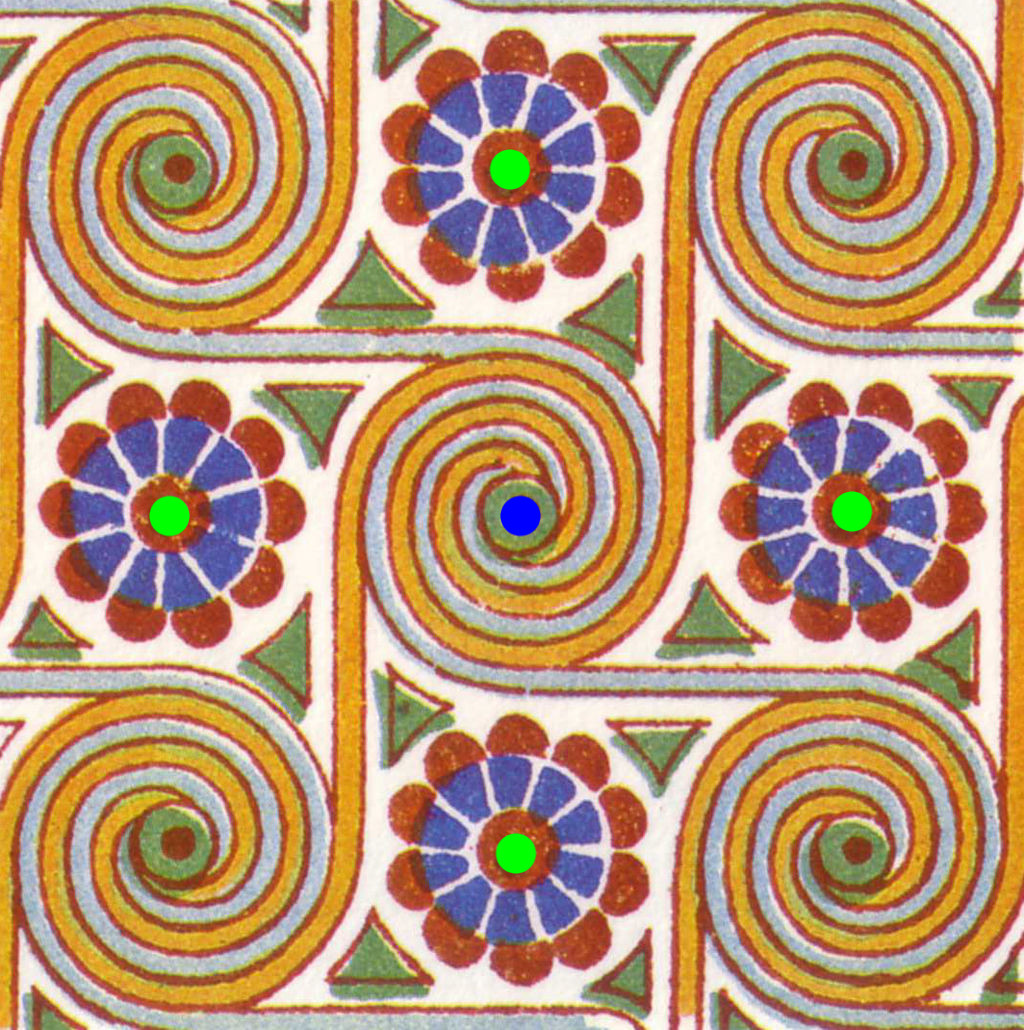
\includegraphics[width=\textwidth]{images/p4_symmetry_wallpaper_E.jpg}
        \caption{Rotational Symmetry}
        \label{fig:rot_sym}
        \end{subfigure}
        \begin{subfigure}{0.2\textwidth}
            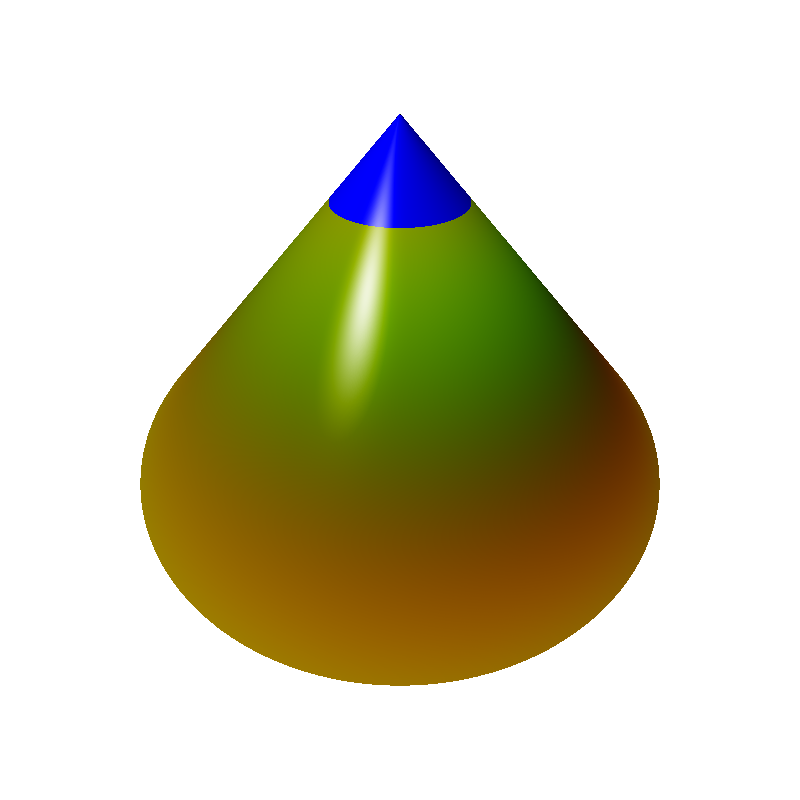
\includegraphics[width=\textwidth]{images/cone_point.png}
            \caption{Cone Point}
            \label{fig:cp}
        \end{subfigure}
        \begin{subfigure}{0.25\textwidth}
        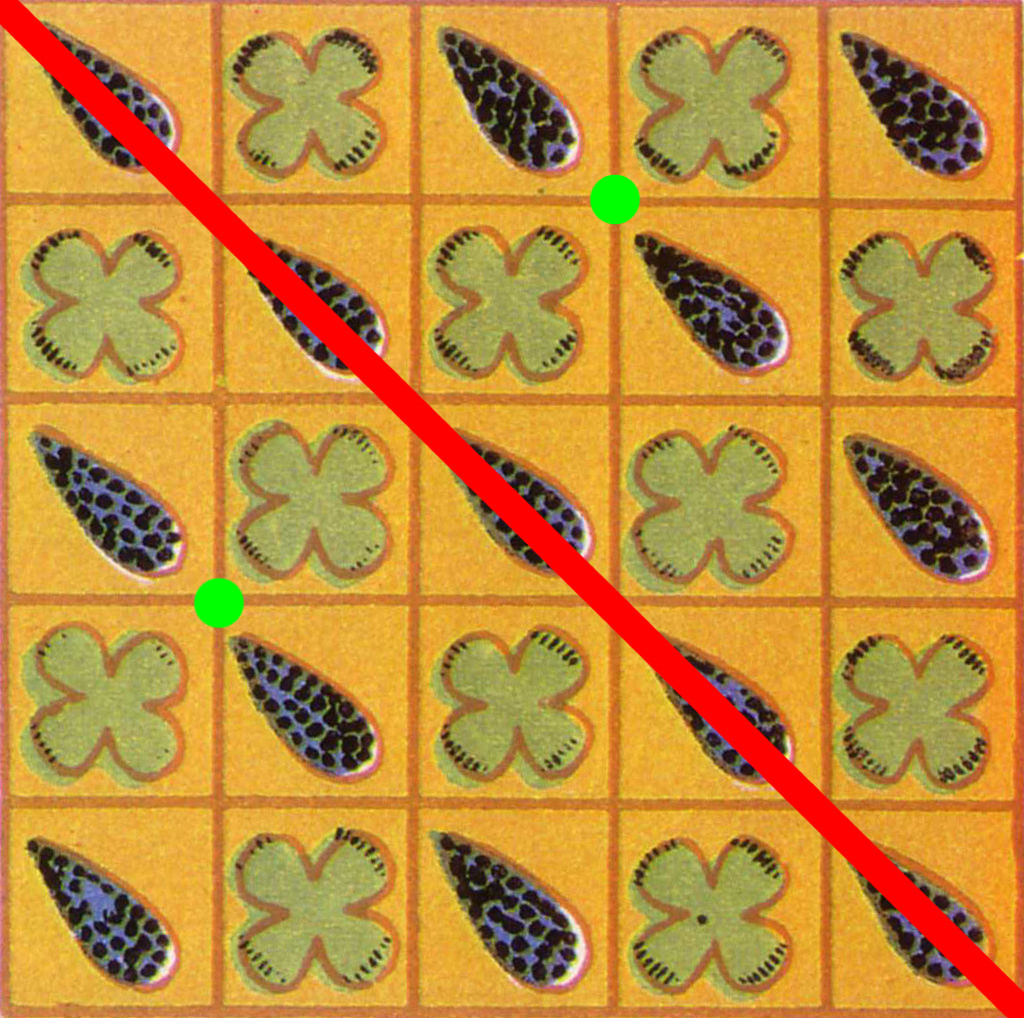
\includegraphics[width=\textwidth]{images/reflection_symmetry_wallpaper_E.jpg}
        \caption{Reflectional Symmetry}
        \label{fig:ref_sym}
        \end{subfigure}
        \begin{subfigure}{0.2\textwidth}
            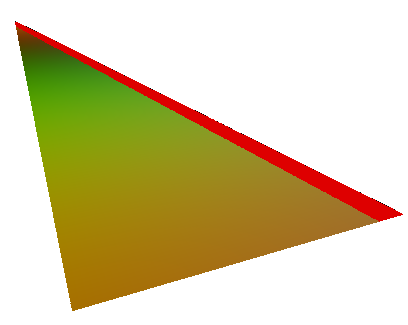
\includegraphics[width=\textwidth]{images/mirror_edge.png}
            \caption{Mirror Edge}
            \label{fig:me}
        \end{subfigure}
        \caption{Folding Symmetries}
        \label{fig:sym}
    \end{figure}

%\begin{figure}[h]
%\centering
%\begin{subfigure}{.2\textwidth}
%  \centering
%  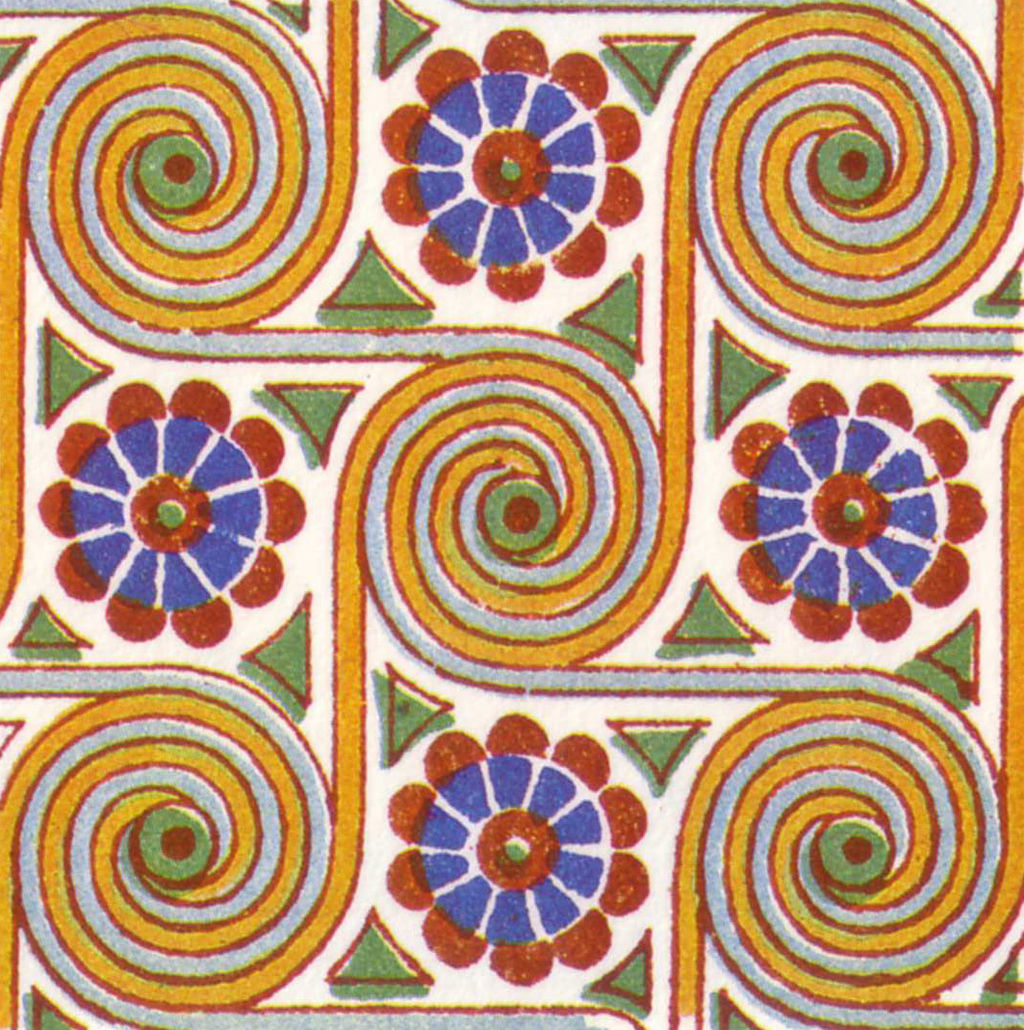
\includegraphics[width=0.9\linewidth]{images/p4_symmetry_wallpaper.jpg}
%  %\caption{A subfigure}g
%  \label{fig:sub1}
%\end{subfigure}%
%\begin{subfigure}{.2\textwidth}
%  \centering
%  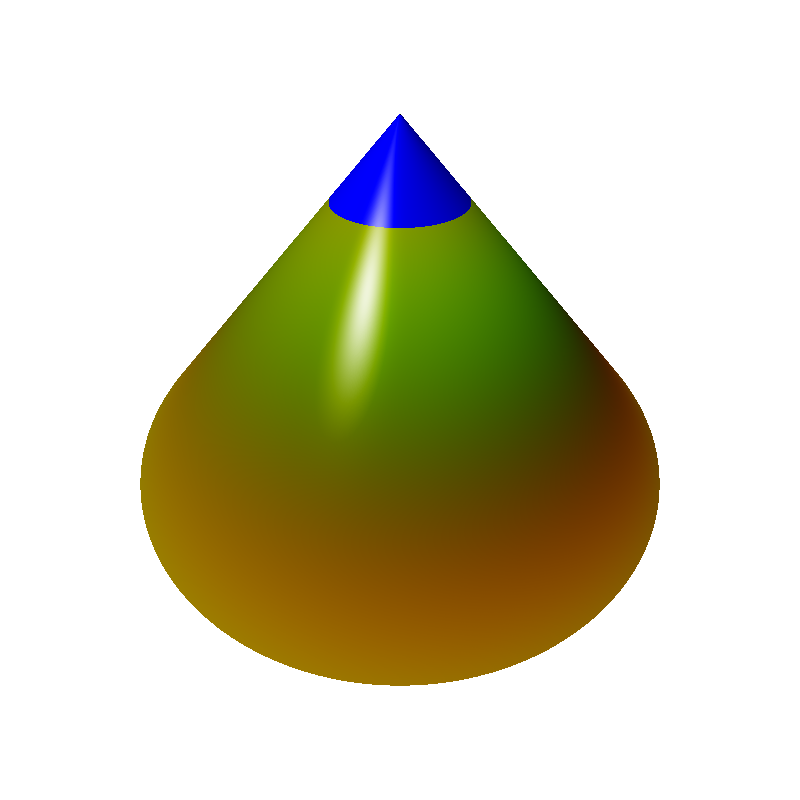
\includegraphics[width=0.9\linewidth]{images/cone_point.png}
%  %\caption{A subfigure}
%  \label{fig:sub2}
%\end{subfigure}
%\label{fig:sym}
%\end{figure}

Finally, an orbifold is a generalization of a simple $n$ dimensional surface,
which we call a manifold. While a manifold allows local structure of flat
space $\mathbb{R}^n$, an orbifold allows local structure of the quotient
space of $\mathbb{R}^n$ with respect to some group. So, for every small
neighborhood on the surface of an orbifold, there exists a corresponding
group and some strata. A visual representation of a two dimensional
orbifold is shown in Figure~\ref{fig:orb}. Note the red represents mirror
edge strata and the blue represents cone point strata.

\begin{figure}
\centering
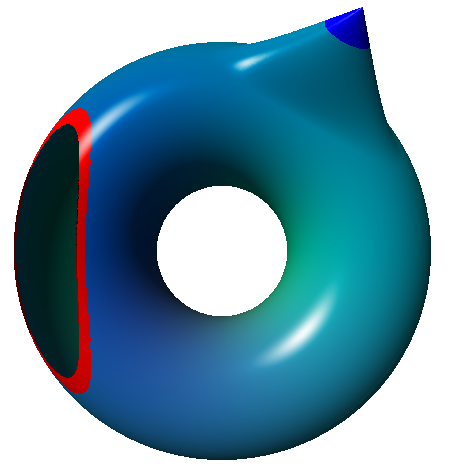
\includegraphics[width=0.3\textwidth]{images/orbifold_ex.png}
\caption{Orbifold Visualization}
\label{fig:orb}
\end{figure}

\section{Laplace Spectra}
In order to formalize the notion of ``sound'' we introduce the notion of
the Laplace Spectra, which mathematically represents the frequencies of
vibrations of a particular object. We define the Laplace Spectra as
follows (note the symbol $\Delta$ represents the Laplacian operator).
Motivated by conservation of energy and the fact that resonance frequencies
correspond to standing waves, we can define the function $\psi(\mathbf{x})$
such that it outputs the amplitude of some specific standing wave on some
surface at any coordinate vector $\mathbf{x}$ on the surface.  Then,
motivated by conservation of energy, we can show that the solutions for
$\lambda$ in the equation $\Delta \psi(\mathbf{x}) = -\lambda
\psi(\mathbf{x})$ are closely related to the physical notion of resonance
frequencies. We call the full sequence of eigenvalue solutions $\lambda_1,
\lambda_2, \dots$ the \emph{Laplace Spectra}. For a physical object, we can
consistently relate the Laplace Spectra of an object to the physics notion
of resonant frequencies. Importantly, we can apply this formal notion of
sound to mathematical abstractions such as orbifolds.

\section{Research Question}
Intuitively, our research question is, can you hear the shape of an
orbifold.  But we can now state our research question more precisely. In
this research project, we ask: Given the Laplace Spectra of some orbifold,
what properties can we deduce about the orbifold?

\section{Result}

The major result of this research project is a new definition paired with a
theorem. Our definition of the new term local orientability is as follows:

\begin{definition}[Local Orientability]
A small local neighborhood with group $\Gamma$ on some orbifold is \emph{orientable} if 
all elements $\Gamma$ are orientation-preserving transformations. An
orbifold $\mathcal{O}$ is \emph{locally orientable} if every chart on
$\mathcal{O}$ is orientable.  Conversely, an orbifold $\mathcal{O}$ is
\emph{locally non-orientable} if there exists a single chart on
$\mathcal{O}$ that is not orientable.
\end{definition}

\begin{theorem*}
    A locally orientable orbifold and a locally non-orientable orbifold
    will have a different Laplace Spectra. Or, you can hear the local
    orientability of an orbifold.
\end{theorem*}

 Simply put, we proved that orbifolds with a group containing
orientation-reversing operations will always have a different Laplace
Spectra than orbifolds that have no such group. Below we represent two
orbifolds that this theorem guarantees have different Laplace Spectra.

\begin{figure}[h]
    \centering
        \begin{subfigure}{0.25\textwidth}
            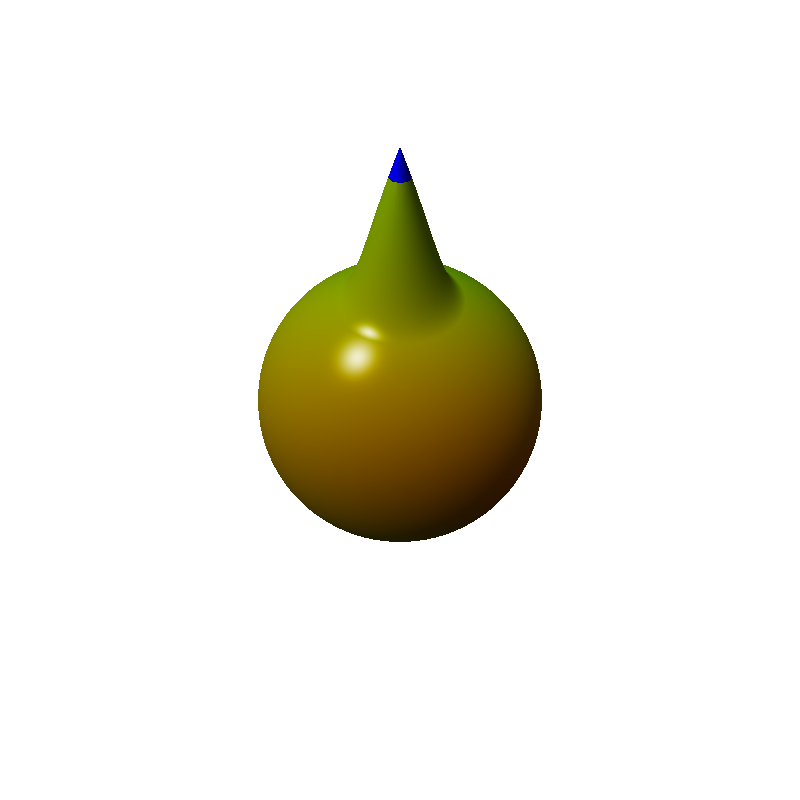
\includegraphics[width=\textwidth]{images/teardrop.png} 
        \end{subfigure}
        \begin{subfigure}{0.25\textwidth}
            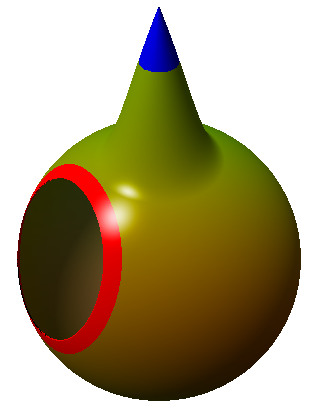
\includegraphics[width=\textwidth]{images/teardrop_edge.png}
        \end{subfigure}
        \caption{Non-isospectral Orbifolds}
        \label{fig:result_ex}
    \end{figure}

\section{Asymptotic Heat Expansion}
To approach this problem, we use the asymptotic heat expansion technique as
discussed in the paper \textit{Asymptotic Expansion of the Heat Kernel for
Orbifolds}. In approximating how heat moves through the orbifold, we obtain
a polynomial of the form $H(t) = \sum_{k=-\dim(\orb)}^{\infty} h_{k/2}
t^{k/2}$. Every orbifold has a such a polynomial. 
Importantly, \textit{Asymptotic Expansion} demonstrates that two orbifolds
have the same Laplace Spectra exactly when the orbifolds have the same heat
expansion.

In combining 4.5, 4.7, and 4.8 in \textit{Asymptotic Expansion} we have
that an orbifold $\orb$ with collection of strata $S(\orb)$ has the
following heat expansion:

\begin{align*}
    H(t) = {(4\pi t)}^{-\dim(\mathcal{O})/2}\sum_{k=0}^{\infty}a_k(\mathcal{O})t^k
            +\sum_{N \in S(\mathcal{O})}\frac{{(4\pi t)}^{-\dim(N)/2}}{\myabs{\iso(N)}}\sum_{k=0}^{\infty}t^k\int_{N} \sum_{\gamma \in \iso^{\max}(\tilde{N})}b_k(\gamma,x) dvol_N
\end{align*}

There are a few important take-aways from this formula. 
Without loss of generality, we study odd dimensional orbifolds.
Firstly, the strata in the orbifold affect the expansion.  Importantly, for
an odd dimension orbifold, the only way for an expansion to have a non-zero
$t^{k}$ term where $k$ is some integer is by containing some \emph{even
dimensional strata}. This fact is essential in proving the result.

\section{Intuitive Proof}

A substantial amount of 

\begin{proof}

Take $\mathcal{O}_o$ to be a locally orientable orbifold and
$\mathcal{O}_n$ to be a locally non-orientable orbifold. Then, we claim
that $\mathcal{O}_o$ and $\mathcal{O}_n$ have different Laplace Spectra. 

It is known that orbifolds of different dimensions have different Laplace
Spectra /*citation needed*/, thus we conclude $\dim(\orb_o) =
\dim(\orb_n)$. Without loss of generality, we take this dimension to be
odd.

We now consider the asymptotic heat expansion of $\orb_o$ and $\orb_n$. We
can argue that the orbifold has an even dimensional strata if and only if
it is locally non-orientable. Verifying this argument is technical
/*briefly cite Donnely?*/, but
this essential states that out three dimensional world, we only have two
dimensional mirrors. Then, if no even dimension strata exists in $\orb_o$,
every integer power coefficient in $\orb_o$ is zero.

Conversely, the even dimensional strata in $\orb_n$ contribute to to the
whole power coefficients. We summarize, the possible heat expansion coefficients
below.

\begin{figure}[h]
\centering
\begin{tabular}{c | c c c c c c c}
    & \dots & $t^{-1}$ & $t^{-1/2}$ & $t^{0}$ & $t^{1/2}$ & $t^{1}$ & \dots\\
\hline
$\mathcal{O}_o$ &
    \dots & $0$ & $\#$ & $0$ & $\# $& $0$ & \dots \\
$\mathcal{O}_n$ &
\dots & $d_{-1}$ & $\#$ & $d_0$ & $\# $& $d_1$ & \dots  \\
\end{tabular}
\caption{Heat expansion coefficients}
\end{figure}
We aim to show that at least one $d_i$ is non-zero. We can show that for a
specific strata, the strata is guaranteed to contribute a strictly positive
amount to the $t^k$ for the most negative $k$ the strata applies to. Then,
in considering the strata of maximal dimension, we know there exists at
least one strictly positive $d_i$ term. Thus, $O_o$ and $O_n$ have
different asymptotic heat expansion, so $O_o$ and $O_n$ have different
Laplace Spectra. This concludes the proof that locally orientable and
locally non-orientable orbifolds have different Laplace Spectra.
\end{proof}

\citation{DUMMY:1}

\bibliography{sample}

%\begin{thebibliography}
%    \bibitem{SOT}
%    test
%
%%\\
%%/*symmetries of things*/ \\
%%/*DGGW (asympt expansion...)*/\\
%%/*Can you hear the shape of a drum article*/\\
%%/*Donnely?*/
%\end{thebibliography}

\end{document}
